\documentclass[aspectration=1610,t]{beamer}
\usepackage{csc}
\title{Лекция 1. OpenGL --- база}


\date{
   \textbf{ИТМО}\\
   14 сентября 2022\\
   Санкт-Петербург
}

\begin{document}

\begin{frame}
  \titlepage
\end{frame}

\begin{frame}[fragile]{Некоторые вводные}
    Ожидается, что люди, пришедшие на курс:
    \begin{itemize}
        \item имеют опыт программирования на языках \langc/\langcpp.
        \item способны читать документацию на английском языке.
    \end{itemize}
\end{frame}

\begin{frame}[fragile]{Что будет в лекции}
    \begin{itemize}
        \item Рассказ про {\bf OpenGL Context}.
        \item Расширения (extensions).
        \item OpenGL {\bf Сore} vs {\bf Сompatibility} profile.
        \item {\bf Вершинный} и {\bf индексный} буферы OpenGL.
        \item Шейдерные программы: {\bf Vertex} и {\bf Fragment}.
        \item {\bf Атрибуты} (attributes) и {\bf юниформы} (uniforms).
        \item Шаблон приложения с использованием библиотеки QT.
    \end{itemize}
\end{frame}

\begin{frame}[fragile]{Где искать ответы на вопросы}
    \begin{itemize}
        \item Вопросы и ответы \url{https://stackoverflow.com}.
        \item Спецификация на \url{https://www.khronos.org/registry/OpenGL/specs/gl/glspec33.core.pdf/}.
        \item Все спецификации + расширения \url{https://www.khronos.org/registry/OpenGL/index_gl.php}
        \item Уроки на \url{https://learnopengl.com/}.
        \item Переводы части уроков на \url{https://habr.com/ru/post/310790/}.
    \end{itemize}
\end{frame}

\begin{frame}[fragile]{Почему OpenGL 3.3?}
    \begin{itemize}
        \item Все основные функции уже реализованы.
        \item Новые версии только добавляют полезные возможности,
            не~изменяя принципов работы с графическим API.
        \item {\bf 3.3}~--- версия, которая запустится на практически 
            любом графическом ускорителе.
        \item Дополнительные возможности можно получить с помощью расширений.
    \end{itemize}
\end{frame}

\begin{frame}[fragile]{Расширения OpenGL}
    \begin{itemize}
        \item Производители графических карт могут дополнять функционал графического API.
        \item Популярные, как правило, попадают в новые версии API.
        \item Существует механизм для работы с расширениями в run-time.
            Выглядит это примерно так:
            {\small \begin{lstlisting}
if (extension exists) {
    // call new API
}
else {
    // use old one
}
            \end{lstlisting}}
    \end{itemize}
\end{frame}

\begin{frame}[fragile]{Core VS Compatibility}
    \begin{itemize}
        \item Использование {\bf Core}-профиля заставляет нас 
            пользоваться современными и актуальными практиками 
            при разработке графических приложений.
        \item {\bf Compatibility}-профиль сохраняет совместимость.
    \end{itemize}
    Замечание: на некоторых платформах {\bf Compatibility} 
    не доступен (например, на платформах Apple).
\end{frame}

\begin{frame}[fragile]{OpenGL Сontext и его состояние}
    \begin{itemize}
        \item OpenGL по своей сути — это {\bf большой конечный автомат}: набор переменных, 
            определяющий некоторое состояние.
        \item Перед отрисовкой следующего кадра мы задаем необходимое {\bf состояние}, 
            которое говорит OpenGL, {\bf как нужно рисовать}.
        \item Под состоянием графического конвейера обычно имеют ввиду состояние контекста.
    \end{itemize}
\end{frame}

\begin{frame}[fragile]{Основные шаги для отрисовки}
    \begin{itemize}
        \item Подготовливаем сцену (в геометрическом смысле).
        \item Создаем и заполняем необходимые OpenGL-буферы, копируем их в видеопамять.
        \item Задаем необходимое состояние контекста (как рисуем + куда рисуем).
        \item Делаем вызов отрисовки.
        \item {\bf ВАЖНО}: освобождаем не нужные более нам ресурсы.
    \end{itemize}
    Далее рассмотрим эти шаги подробнее.
\end{frame}

\begin{frame}[fragile]{Подготовка сцены}
    \begin{itemize}
        \item Обновляем объекты в сцене.
        \item Выполняем предварительные вычисления видимости, 
            т.е.~определяем, что попало в сцену, чтобы не рисовать лишние объекты.
        \item Возможно, обрабатываем пользовательские события.
        \item \dots
    \end{itemize}
    В результате должны получить набор объектов \langcpp, 
        которые будем использовать для формирования буферов в видеопамяти.
\end{frame}

\begin{frame}[fragile]{Буферы OpenGL}
    \begin{itemize}
        \item OpenGL~--- преимущественно \langc~-библиотека, 
            поэтому работа со~всеми объектам осуществляется в стиле \langc.
        \item Создать объект в видеопамяти значит заполнить некоторую \langc~-структуру,
            которая в дальнейшем будет записана в~видеопамять.
    \end{itemize}
\end{frame}

\begin{frame}[fragile]{Буферы OpenGL}
    Общая схема работа с объектами в OpenGL:
        {\small \begin{lstlisting}
GLuint object_id = 0;
glGenObject(1, &object_id);
glBindObject(object_id);
glSetObjectStateOrData(...);
glBindObject(0);
        \end{lstlisting}}
\end{frame}

\begin{frame}[fragile]{Вершинный буфер}
    \begin{itemize}
        \item Содержит геометрию вершин и их атрибуты.
        \item По сути~--- набор байтов.
        \item Чтобы OpenGL смог их корректно прочитать, нужно задать правильные смещения.
        \item Такие буферы обычно называют {\bf VBO} (Vertex Buffer Object).
    \end{itemize}
\end{frame}

\begin{frame}[fragile]{Создание вершинного буфера}
    \begin{itemize}
        \item Зададим геометрию:
            {\small \begin{lstlisting}
GLfloat vertices[] = { // треугольник из 3 вершин
    -0.5f, -0.5f, 0.0f,
    0.5f, -0.5f, 0.0f,
    0.0f,  0.5f, 0.0f
};
            \end{lstlisting}}
        \item Создадим и заполним объект в видеопамяти:
            {\small \begin{lstlisting}
GLuint vbo;
glGenBuffers(1, &vbo);
glBindBuffer(GL_ARRAY_BUFFER, vbo);
glBufferData(GL_ARRAY_BUFFER, sizeof(vertices),
             vertices, GL_STATIC_DRAW);
            \end{lstlisting}}
    \end{itemize}
\end{frame}

\begin{frame}[fragile]{Создание вершинного буфера}
    Режимы отрисовки.
    \begin{itemize}
        \item GL\_STATIC\_DRAW~--- данные редко изменяются в памяти.
        \item GL\_DYNAMIC\_DRAW~--- данные изменяются часто.
        \item GL\_STREAM\_DRAW~--- данные изменяются на каждый кадр.
    \end{itemize}
    Это позволяет оптимально использовать видеопамять.
\end{frame}

\begin{frame}[fragile]{Разметка вершинных атрибутов}
    \begin{itemize}
        \item Формат вершин:
            \begin{figure}[htp]
                \centering
                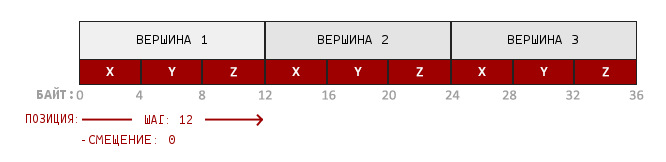
\includegraphics[scale=0.45]{vertex_attributes}
            \end{figure}
        \item Разметка:
            {\small \begin{lstlisting}
glVertexAttribPointer(0, 3, GL_FLOAT, GL_FALSE,
                      3 * sizeof(GLfloat), 0);
glEnableVertexAttribArray(0);
            \end{lstlisting}}
    \end{itemize}
\end{frame}

\begin{frame}[fragile]{Разметка вершинных атрибутов}
    Аргументы {\bf glVertexAttribPointer}:
    \begin{enumerate}
        \item Какой аргумент шейдера хотим настроить (location).
        \item Размер аргумента шейдера, в нашем случае vec3.
        \item Тип данных~--- GL\_FLOAT.
        \item Нужно ли нормализовать данные.
        \item Размер вершины.
        \item Смещение от начала буфера.
            {\small \begin{lstlisting}
glVertexAttribPointer(0, 3, GL_FLOAT, GL_FALSE,
                      3 * sizeof(GLfloat), 0);
glEnableVertexAttribArray(0);
            \end{lstlisting}}
    \end{itemize}
\end{frame}

\begin{frame}[fragile]{Индексный буфер}
    \begin{itemize}
        \item Содержит индексы вершин из вершинного буфера.
        \item Такие буферы обычно называют {\bf IBO} (Index Buffer Object) 
            или {\bf EBO} (Element Buffer Object).
    \end{itemize}
\end{frame}

\begin{frame}[fragile]{Создание индексного буфера}
    \begin{itemize}
        \item Зададим индексы:
            {\small \begin{lstlisting}
GLuint indices[] = { // треугольник из 3 вершин
    0, 1, 2
};
            \end{lstlisting}}
        \item Создадим и заполним объект в видеопамяти:
            {\small \begin{lstlisting}
GLuint ibo;
glGenBuffers(1, &ibo);
glBindBuffer(GL_ELEMENT_ARRAY_BUFFER, ibo);
glBufferData(GL_ELEMENT_ARRAY_BUFFER,
             sizeof(indices), indices,
             GL_STATIC_DRAW);
            \end{lstlisting}}
    \end{itemize}
\end{frame}

\begin{frame}[fragile]{Vertex Array Object}
    Некоторая обертка, позволяющая быстро переиспользовать VBO~и IBO.
    \begin{figure}[htp]
        \centering
        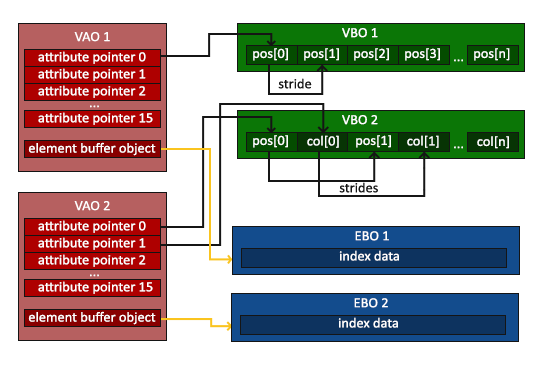
\includegraphics[scale=0.40]{vao}
    \end{figure}
\end{frame}

\begin{frame}[fragile]{Шейдерные программы}
    \begin{itemize}
        \item Соотвествуют специальным программируемым частям конвейера.
        \item Пишутся на \langc-подобном языке~--- {\bf GLSL}.
        \item Требуют дополнительной компиляции.
        \item Вершинный шейдер обрабатывает каждую вершину.
        \item Фрагментный шейдер~--- каждый фрагмент (в каком-то смысле пиксель).
    \end{itemize}
\end{frame}

\begin{frame}[fragile]{Вершинный шейдер}
    Пример вершинного шейдера:
    {\small \begin{lstlisting}
#version 330 core

layout (location = 0) in vec3 vertex_position;

void main()
{
    gl_Position = vec4(vertex_position.xyz, 1.0);
}
    \end{lstlisting}}
\end{frame}

\begin{frame}[fragile]{Вершинный шейдер}
    Создание вершинного шейдера:
    {\small \begin{lstlisting}
GLuint vs = glCreateShader(GL_VERTEX_SHADER);
glShaderSource(vs, 1, &vs_source, 0);
glCompileShader(vs);
    \end{lstlisting}}
\end{frame}

\begin{frame}[fragile]{Фрагментный шейдер}
    Пример фрагментного шейдера:
    {\small \begin{lstlisting}
#version 330 core

out vec4 fragment_color;

void main()
{
    fragment_color = vec4(1.f, 0.f, 0.f, 1.f);
}
    \end{lstlisting}}
\end{frame}

\begin{frame}[fragile]{Фрагментный шейдер}
    Создание фрагментного шейдера:
    {\small \begin{lstlisting}
GLuint fs = glCreateShader(GL_FRAGMENT_SHADER);
glShaderSource(fs, 1, &fs_source, 0);
glCompileShader(fs);
    \end{lstlisting}}
\end{frame}

\begin{frame}[fragile]{Шейдерная программа}
    Соотвествует набору шейдеров.
    {\small \begin{lstlisting}
GLuint sp = glCreateProgram();
glAttachShader(sp, vs);
glAttachShader(sp, fs);
glLinkProgram(sp);
    \end{lstlisting}}
    Замечание: если шейдер не задан, то он заменяется шейдером по~умолчанию.
\end{frame}

\begin{frame}[fragile]{Подготовка к отрисовке}
    Задаем буферы для отрисовки:
    {\small \begin{lstlisting}
glBindVertexArray(vao);
glBindBuffer(GL_ARRAY_BUFFER, vbo); 
glBufferData(GL_ARRAY_BUFFER, sizeof(vertices),
                vertices, GL_STATIC_DRAW); 
glVertexAttribPointer(0, 3, GL_FLOAT, GL_FALSE,
                        3 * sizeof(GLfloat), 0);
glEnableVertexAttribArray(0);
glBindVertexArray(0);
    \end{lstlisting}}
\end{frame}

\begin{frame}[fragile]{Отрисовка}
    Сначала зададим шейдерную программу и VAO:
    {\small \begin{lstlisting}
glUseProgram(sp); 
glBindVertexArray(vao); 
    \end{lstlisting}}
    Отрисуем треугольник:
    {\small \begin{lstlisting}
glDrawElements(GL_TRIANGLES, 3, GL_UNSIGNED_INT, 0)
glBindVertexArray(0);
    \end{lstlisting}}
\end{frame}

\begin{frame}[fragile]{Unifroms}
    \begin{itemize}
        \item Юниформы~--- некоторые глобальные для всей шейдерной программы переменные.
        \item Задаются из пользовательского кода на \langcpp.
        \item Используются в шейдере при помощи ключевого слова {\bf uniform}. Например:
            {\small \begin{lstlisting}
#version 330 core
out vec4 color;

uniform vec4 u_color;

void main()
{
    color = u_color;
}
            \end{lstlisting}}
    \end{itemize}
\end{frame}

\begin{frame}[fragile]{Unifroms}
    Как задать uniform из кода?
    \begin{itemize}
        \item Сначала узнаем расположение:
            {\small \begin{lstlisting}
GLint color_location;
color_location = glGetUniformLocation(sp,
                                      "u_color");
            \end{lstlisting}}
        \item Потом задаем значение:
            {\small \begin{lstlisting}
glUseProgram(sp);
glUniform4f(color_location, 1.f, 0.f, 0.f, 1.f);
            \end{lstlisting}}
    \end{itemize}
\end{frame}

\begin{frame}[fragile]{Обработка ошибок}
    \begin{itemize}
        \item Обработка ошибок происходит в стиле \langc.
        \item Для получения статусов используются функции вида {\bf glGet*}. 
            Например, для шейдеров:
            {\small \begin{lstlisting}
GLint status;
glGetShaderiv(vs, GL_COMPILE_STATUS, &status);
            \end{lstlisting}}
        \item Также существует функция {\bf glGetError}, 
            которая возвращает информацию об ошибках.
    \end{itemize}
\end{frame}

\begin{frame}[fragile]{Корректное управление ресурсами}
    \begin{itemize}
        \item Все созданные OpenGL объекты должны быть освобождены вручную.
        \item Инициализация объектов должна производиться единожды.
        \item Заполнять и модифицировать эти объекты можно бесконечно много раз.
        \item Заполнять данные нужно только по мере их изменения.
    \end{itemize}
\end{frame}

\end{document}

